\documentclass[0-thesis.tex]{subfiles}

\begin{document}
\label{chap:profiles}
The previous two sections have proposed a technology agnostic update architecture and a
life cycle perspective for devices. It is time to show concrete incarnations of this
architecture using state of the art IoT protocols. This section is aimed towards
implementers needing to make decisions about how to implement the update architecture.
This section will discuss choice of image digest algorithm, vendor and class ID
generation, payload encoding and encryption, and considerations when choosing between
DTLS/CoAP and OSCORE for an update architecture profile.

\subsection{DTLS Profile}
\label{ssec:dtls-profile}
When implementing the architecture, one choice of protocols is using DTLS and CoAP for
constrained communication to and from devices. For enrollment and authorization, EST and
ACE can be used with their respective suitable profiles. However, as DTLS provides
security at the transport layer it cannot be used for broadcasting, OSCORE is an
option better suited for broadcasting. Note that the architecture itself is broadcast
friendly as it does not make security assumptions that would break broadcasting, but
choice of protocols will influence the viability of broadcasting.

DTLS is already profiled for use in IoT contexts and EST and ACE profiles are works in
progress \parencite{rfc7925, est-coaps, ace-dtls-profile}. The update architecture needs
little extra profiling in addition to these protocols, namely image digest algorithm,
vendor and class ID generation, payload encoding, and payload encryption. The security of
the architecture is not bound to characteristics of any of these protocols and others can
be used instead, this is just one possible profile.

Figure~\ref{fig:dtls-profile} shows where in the constrained part of architecture the
different protocols of the DTLS profile will be used. All communication to and from the
device is reliant on DTLS, the only exception is the enrollment procedure which will
require a pre-shared key as discussed in Section~\ref{ssec:key-management}. The
communication protocols in the non-constrained part of the architecture are suggestions
and not part of the profile.

\begin{figure}[t]
    \caption{The various protocols used in the DTLS profile. Protocols outside the constrained networks are suggestions.}
    \label{fig:dtls-profile}
    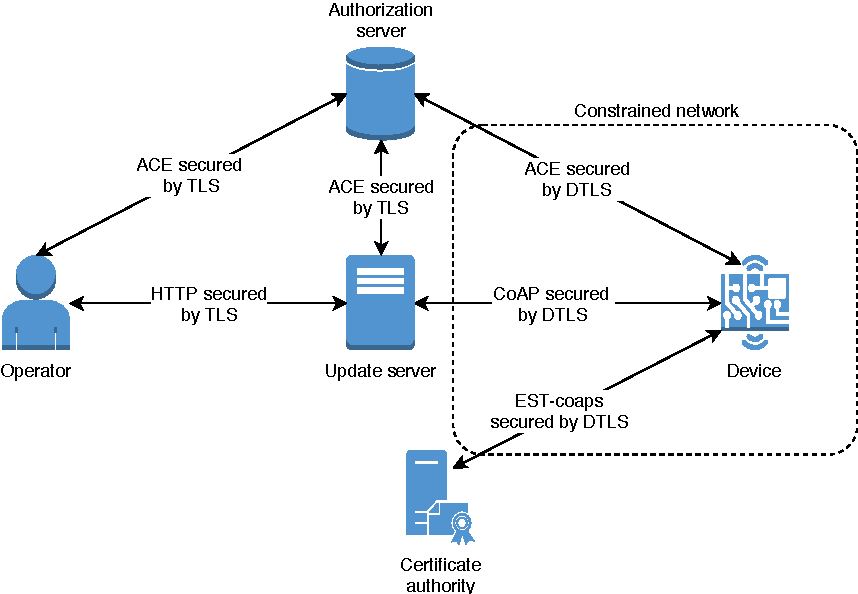
\includegraphics{images/dtls-profile.pdf}
\end{figure}

\subsubsection{ID Generation and Hash Algorithms}
\label{sssec:hash-id-algorithm}
The DTLS IoT profile suggests ciphersuites for the use of pre-shared keys and certificates
and EST has been profiled with CoAPs to use the same ciphersuites for certificates. These
suites implement the \textbf{SHA-256} hash function which can be used to calculate the
digest of an image. Since the digest is just supposed to verify the integrity of the
image, SHA-256 is an adequate choice and does not require implementing new hash algorithms
for devices already running DTLS.

Generating vendor and class IDs should be done so that devices get unique identifiers and
devices with the same names from different vendors do not clash. For this purpose,
\textbf{UUIDs} can be used \parencite{rfc4122}. Version 3 and 5 of UUID are "name-based"
versions meaning they operate in a given namespace. By using a registered domain name of
the vendor, which is already guaranteed to be unique, as namespace a unique UUID can be
generated for that vendor. By using the vendor UUID as the namespace for the class IDs,
devices from different vendors can share names but still have different class IDs. A
hierarchical namespace structure is suggested also by SUIT.

Section 4.3 of the UUID specification states that "Choose either MD5 or SHA-1 as the hash
algorithm; If backward compatibility is not an issue, SHA-1 is preferred". This means
\textbf{UUID5} should be used as it uses SHA-1 for hashing. ID generation will not occur
on the devices themselves, devices only need to be prepared with their IDs for comparing
with the manifest.

\subsubsection{Payload Encoding and Encryption}
\label{sssec:encoding-encryption}
For encoding, \textbf{\gls{cbor}} is an efficient binary encoding \parencite{rfc7049}.
CBOR aims to be an extensible data format providing very small code sizes. It supports
simple values as well as arrays and maps meaning it is easy to map to and from JSON while
being more compact than JSON. 

The use of CBOR enables the use of \textbf{\gls{cose}} \parencite{rfc8152}. COSE provides
encryption and signing for CBOR encoded objects, which in the architecture will be the
manifest and image. As DTLS secures the channel, the manifest and image can be signed
using COSE objects to ensure their integrity during transport. 

\subsection{OSCORE Profile}
\label{ssec:oscore-profile}
\acrfull{oscore} provides end-to-end protection for CoAP messages using COSE
\parencite{oscore}. By providing end-to-end encryption CoAP message security is not
terminated at a proxy or update server as with DTLS. If updates are being pushed from an
operator to a device directly, OSCORE can support HTTP/CoAP proxying to secure the entire
transport. The update server will not be able to view or manipulate the protected
contents. As update servers are in addition to transporting updates supposed to act as
update repositories, a decision has to be made how updates are stored on the server. This
is an implementation detail.

Figure~\ref{fig:oscore-profile} shows where in the constrained part of architecture the
different protocols of the OSCORE profile will be used. All communication to and from the
device is reliant on OSCORE, the only exception is the enrollment procedure which will
require a pre-shared key as discussed in Section~\ref{ssec:key-management}. The
communication protocols in the non-constrained part of the architecture are suggestions
and not part of the profile. 

\begin{figure}
    \caption{The various protocols used in the OSCORE profile. Protocols outside the constrained networks are suggestions.}
    \label{fig:oscore-profile}
    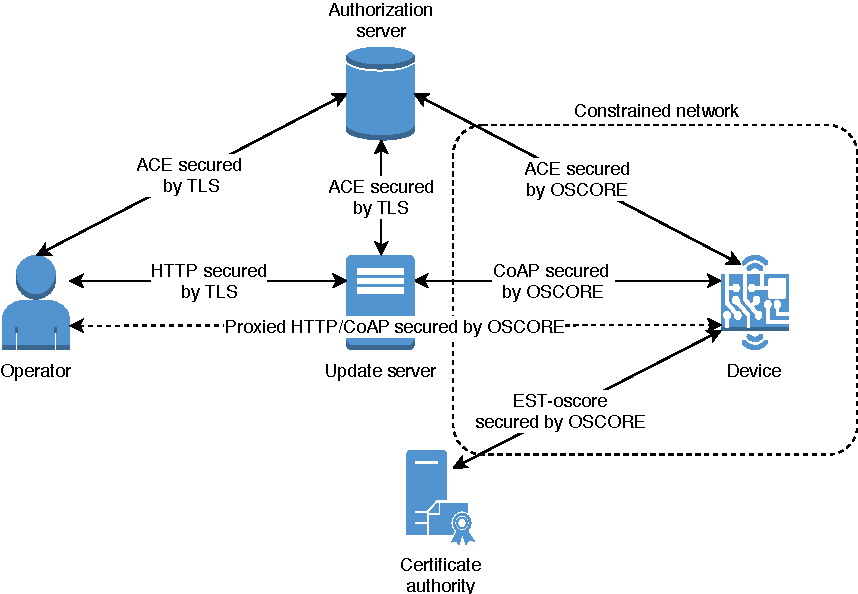
\includegraphics{images/oscore-profile.pdf}
\end{figure}

OSCORE can run directly on top of UDP and supports broadcasting as well as unicast. In the
case of broadcasting, a security context must be defined \parencite{oscore-group}. If a
security context is in place, unicast OSCORE is still possible. At the time of writing,
there are two Internet-Drafts aiming to specify profiles for ACE and EST using OSCORE,
meaning these protocols can be used for enrollment and authorization with OSCORE as well
\parencite{ace-oscore, est-oscore}. ID generation, hash algorithms, and payload encoding
and signing in the OSCORE profile is the same as in the DTLS profile, see
Section~\ref{ssec:dtls-profile}.

When trying to achieve end-to-end encryption key management becomes more difficult, how do
you ensure end-to-end encryption will still allowing all intended recipients (devices) to
decrypt the payload? One solution is to let the operator  encrypt the payload with a
symmetric key which the update server then either encrypts with each intended recipients
asymmetric key or with a group key. This avoids having to re-encrypt the payload (breaking
end-to-end encryption) and allows storing the encrypted payload and just re-encrypting the
key for new recipients. This approach means a trusted communication must be established
between the operator and update server for securely exchanging the symmetric key of the
payload and that update servers must be authorized to retrieve said key.

Another interpretation of end-to-end encryption could be purely between the update server
and devices. If a constrained network possesses some routing capabilities an update server
might not know which intermediaries will be used for transporting a package. In this case,
OSCORE can be used to achieve end-to-end security between the update server and the
intended device, while leaving operator-to-update server communication to some other
security mechanism. This is highly topology dependant.

While being better suited for broadcasting and providing end-to-end security, OSCORE
introduces some key management issues and is not yet standardized. The specification
(\parencite{oscore}) is a work in progress as is many of the profiles mentioned in this
section. DTLS and its related IoT profiles are standardized and much more mature. If
implementing the architecture using OSCORE, it is worth noting the incomplete status of
the standard.

\subsection{Summary}
\label{ssec:profiles-summary}
This section identified two options for implementing the architecture: either CoAP over
DTLS or OSCORE. DTLS does not support broadcasting however which might be of importance,
for this purpose OSCORE can be used instead. OSCORE does not rely on a secure channel
established by DTLS but instead provides end-to-end security for CoAP messages using COSE.
OSCORE is, unlike DTLS, not yet standardized and there is a partial implementation of
OSCORE featuring only COSE encryption objects in a Contiki fork
\parencite{contiki-oscore}. Profiles surrounding DTLS for EST-coaps and ACE are also
closer to standardization than their OSCORE counterparts.

Both profiles use SHA-256 for calculating image digests, UUID5 for vendor and class IDs
using registered vendor domains, EST with its corresponding profile for enrollment, and
ACE with its corresponding profile for authorization. Payloads are encoded and signed
using CBOR and COSE for both approaches, ensuring integrity.

With the proposed profiles, a prototype can be implemented and evaluated. Implementation
of a prototype is the topic of the next chapter.

\end{document}